
\lstset{
	backgroundcolor=\color{lbcolor},
	tabsize=2,
	rulecolor=,
	language=matlab,
        basicstyle=\tiny,
        upquote=true,
        aboveskip={1\baselineskip},
        columns=fixed,
        showstringspaces=false,
        extendedchars=true,
        breaklines=true,
        prebreak = \raisebox{0ex}[0ex][0ex]{\ensuremath{\hookleftarrow}},
        frame=single,
        showtabs=false,
        showspaces=false,
        showstringspaces=false,
        identifierstyle=\ttfamily,
        keywordstyle=\color[rgb]{0,0,1},
        commentstyle=\color[rgb]{0.133,0.545,0.133},
        stringstyle=\color[rgb]{0.627,0.126,0.941},
		numbers=left,
}

\begin{figure}[t]
\lstset{language=C,numbersep=4pt}
\begin{center}
\begin{lstlisting}
	for(int i =0 ; i < 100000; i++)
	{
		a[i] = c[i]*b[i];
	}
\end{lstlisting}
\end{center}
\vspace{-1em}
\captionof{lstlisting}{Very basic loop.}
\label{lst:basic}
\end{figure}

\begin{figure}[t]
    \centering
    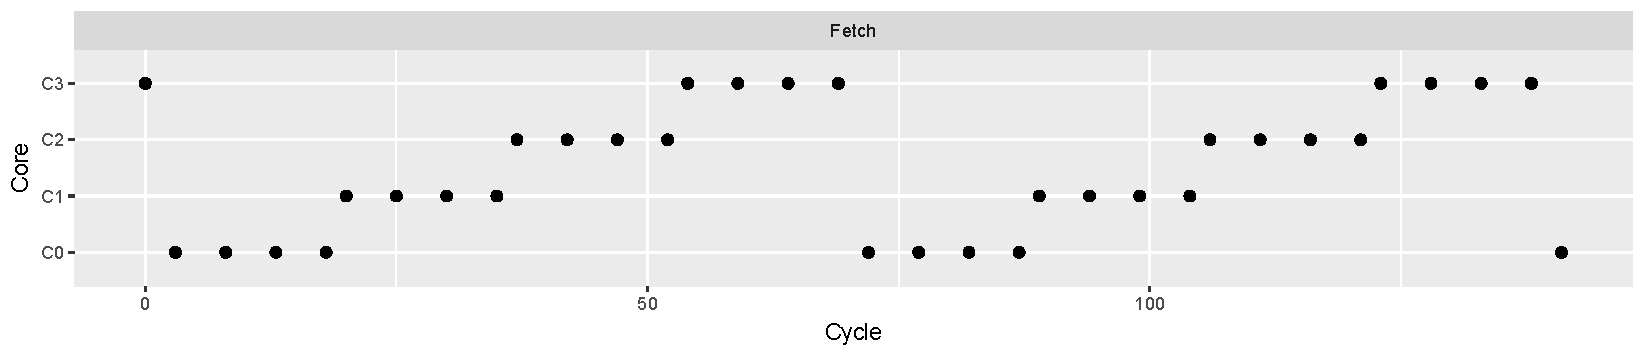
\includegraphics[width=1\textwidth]{chapter3/graphics/4fetchnorm.pdf}
    \caption{Example of the current fetching model on a 2 core composition. Each core has 4 segments, the arrows represent the block generating the predictions. This figure shows the first 5 steps of a new core composition fetching blocks.}
    \label{fig:fetch_norm}
\vspace{1em}
\end{figure}


\subsection{Current fetching scheme}
	
The current block fetching scheme requires that a core fills its instruction window before another core in the composition can fetch a block.
Figure~\ref{fig:old_fetch} illustrates how a two core composition fetches blocks in the current scheme when blocks only take up a single lane of the instruction window.
Once Core 0 is full, it submits a fetch request to Core 1 as seen in Figure~\ref{fig:old_fetch} and stops fetching.
As the figure shows, Core 1 is not active until the 5th fetch request.

The main issue with the current fetching scheme is that cores in a composition depend on each other in order to fetch blocks.
For example, if Listing~\ref{lst:basic} were compiled without unrolling and executed on a 4 core composition, each core would have to fetch 4 iterations before sending the next block request to another core in the composition.

To illustrate how fetching can be a bottleneck, instrumentation was added to the simulator to track when cores fetch blocks in order to be able to visualise how long it takes to fill up a core composition.
Figure~\ref{fig:fetch_norm} plots the when cores fetch blocks for a 4 core composition executing the code in Listing~\ref{lst:basic}.
Each point represents a block fetch, the X-axis represents the time (in cycles) whilst the Y axis represents which core has started fetching a block.
The figure shows that there are 50 cycles between the first block fetched by Core 0 and the first block fetched by Core 3.
Given that a block in Listing~\ref{lst:basic} takes only 10 cycles to execute, this means that Core 0 is innactive when Core 3 fetches.
This is due to the fact that once Core 0 submits a fetch request to Core 1, it will have to wait for Core 3 to send it a fetch request.

Having a serialised block fetching scheme for core composition is one of the main bottlenecks for performance when the compiler cannot produce large blocks.
This means that core composition is not an efficient method of executing blocks in parallel, compared to using multithreading.
Indeed, in a multi-threaded system, cores can fetch blocks independently and thus maximize throughput easily.
A mechanism that can alleviate communication between cores is a first step in improving block throughput for core-compositions.


Fetching blocks in a serial fashion currently makes large core compositions more difficult to use efficiently.
Whilst serialising fetches aims to improve the efficiency of a single core by ensuring that its instruction window is full, it makes populating large core compositions a challenging task.
If cores could fetch blocks independently, this would allow larger core compositions to populate cores in a much quicker fashion.

This section therefore demonstrates how the fetching mechanism can be modified to allow for cores to fetch blocks in parallel.
It starts with a generalised version of the fetching algorith for \textit{n} cores in a composition.
This is followed by a more in-detail example using a two core composition.
Finally it compares the performance of the new fetching scheme with the current fetching scheme on a synthetic benchmark.

\subsection{New fetching mechanism}

\subsubsection{Generalised Form}


The new fetching scheme has two main design objectives: reduce communication amongst cores and ensure that each core in the composition is executing at least one block.
To ensure that each core has at least one block, the composition can be approached as a pipeline.
Sequential blocks should not be found on the same core, instead they should all be on separate cores.
This ensures a more equal distribution of work amongst all the cores in the composition, and also reduces the overhead of populating every core.

Currently, if a core does not have a block in its instruction window, it waits until another core in the composition sends it a fetch request.
If blocks are distributed equally amongst all cores using a pipeline model, this still means that each core must submit a fetch request to the next core.
However, once a core has a block in its instruction window it can use branch prediction to predict the next block it should fetch without having to communicate with the other cores.
As this new fetchign mechanism employs a pipeline model, this means that a core would not predict the next block to fetch for itself, but instead a block that is of a constant stride in the future. %Woof, need to be clearer.
By allowing cores to fetch blocks in \textit{strides}, instead of sequentially, the new fetching mechanism not only ensures cores have an equal amount of work, but that they can fetch in parallel.

Algorithm~\ref{alg:fetch} explains how the new fetching mechanism works for \textit{n} cores in a composition.
In the general case, when a core fetches $block_i$ it will request a prediction for $block_{i+1}$ and $block_{i+n}$.
It submits a fetch request to the next core in the composition for $block_{i+1}$ if the next core is not already executing a block and attempts to fetch $block_{i+n}$.
When committing $block_i$ (Algorithm~\ref{alg:commit}, the core sets the next core in line to be the non-speculative core.
If the next core in line does not have $block_{i+1}$ due to no prediction having been made, then the committing core will submit the resolved PC.

\begin{algorithm}[t]

\textbf{n} = Number of cores in the composition\\
\textbf{Composition[n]} = Core Composition Array\\
\textbf{branches[2]} = Branch Predictions for current block\\

\While{Program is Executing}
{
\If{LastFetchedBlock not branchPredicted}
{
	branches = prediction[i+1, i+n]
}
\eIf{size(branches) == 2}
{
	\eIf{empty(Composition[currentPosition+1])}
	{
		submitToNextCore(branches[0])\\
		submitToMyself(branches[1])
	}
	{
		submitToMyself(branches[1])\\
	}
}
{
	\If{empty(Composition[currentPosition+1])}
	{
		submitToNextCore(branches[0])\\
	}
}	
}
\caption{Overview of fetching algorithm for \textit{n} cores fused}~\label{alg:fetch}
\end{algorithm}

\begin{algorithm}[t]
\textbf{n} = Number of cores in the composition\\
\textbf{Composition[n]} = Core Composition Array\\

\While{Program is Executing}
{
	\If{block is committing}
	{
		Composition[currentPosition+1] = Non Speculative\;
	}
	\If{not IsBlockRunning(Composition[currentPosition+1], block+1)}
	{
		submitToNextCore(block+1 PC)
	}
}
\caption{Overview of commit stage for \textit{n} cores fused}~\label{alg:commit}
\end{algorithm}


\subsubsection{Example using a two core composition}

\begin{figure}[t]
    \centering
    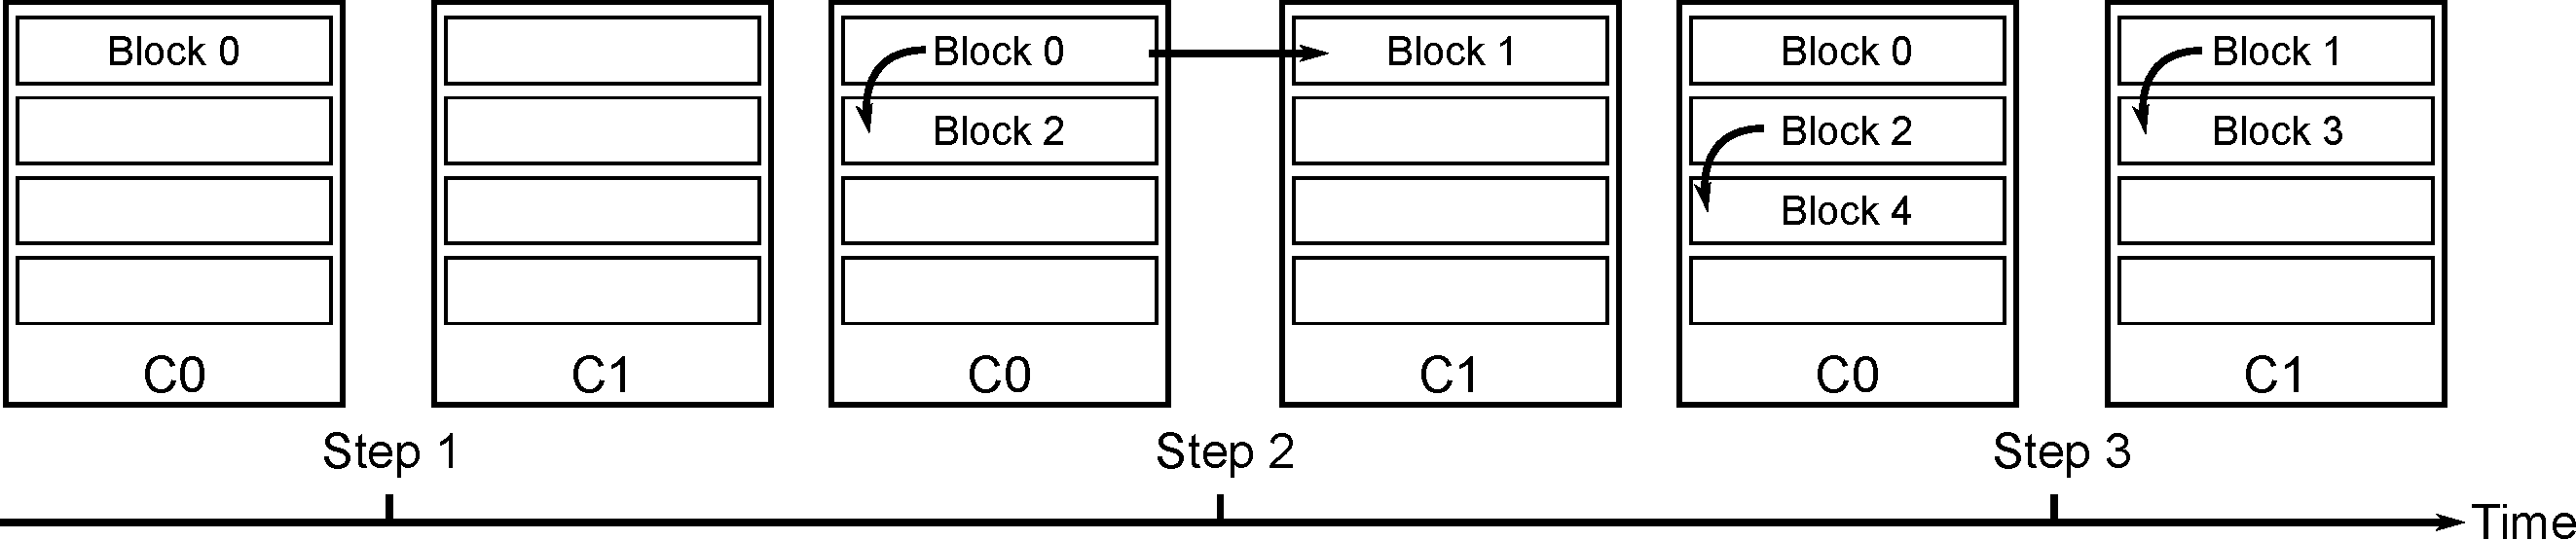
\includegraphics[width=1\textwidth]{chapter3/graphics/fetching-model.pdf}

    \caption{Example of new fetching model on a 2 core composition. Each core has 4 segments, the arrows represent the block generating the predictions. This figure shows the first 3 steps of a new core composition fetching blocks.}
    \label{fig:new_fetch_ex}
\vspace{1em}
	\end{figure}
	
In a core-composition, cores should be able to fetch blocks without requiring a signal from a previous core in the same composition.
Instead, to enable maximum block throughput cores must limit communication to flushes and an initial fetch request.
This allows cores to always be fetching as long as a misprediction hasn't happened.
An initial fetch request is always necessary as only a single core is fetching the first block during a new reconfiguration of the DMP and therefore, other cores must be prompted to fetch at least one block.
However, unlike the current serial model, cores should attempt to submit a fetch signal to the next core in the composition as soon as possible to ensure that all cores are in use.
To understand how the new block mechanism behaves, it will be described in two parts.
The first part will use a concrete example of 2 cores fused, whilst the second part will generalise the mechanism to n-cores fused.

Given a 2 core-fusion \{$Core_0$,$Core_1$\} using a ITTAGE~\cite{SeznecITTAGE} multi-block ahead branch predictor described by A. Seznec et al in~\cite{SeseznecMultipleBlock} the cores can make two predictions in a single cycle: one for itself and one for the next core.
Figure~\ref{fig:new_fetch_ex} gives an overview of the first few cycles of using the new block-fetching scheme with the two cores fused.
When $Core_0$ starts the composition and fetches the first block, $block_0$, if it is able to predict $block_2$ is will submit a fetch request for $block_1$ on $Core_1$ whilst also attempting to fetch $block_2$ for itself.
On the next cycle $Core_1$ receives the request for $block_1$ and starts fetching the block.
Once $Core_1$ can make a branch prediction it will attempt to predict for $block_3$ instead of $block_2$; this is because $block_2$ was already predicted and fetched on $Core_0$.

In this new fetch mechanism, when a core is in fetching mode, it does not attempt to predict $block_{n+1}$ but rather $block_{n+numberOfCoresInComposition}$; the reason behind this will be clarified shortly.
If $Core_0$ or $Core_1$ attempts to fetch a block when it is full, it can submit the new block's PC to a buffer; the core then stops attempting to allocate new blocks.
Once the full Core has committed a block, it checks if it has a buffered PC, and if it does it fetches that block.

As long as $Core_0$ and $Core_1$ can fetch and predict blocks correctly, they will fetch in a pipelined fashion.
This means that $Core_0$ will have blocks \{0,2,4,6\} whilst $Core_1$ has \{1,3,5,7\}.
The reason behind this is to minimize the Synchronization Cost defined in Chapter 2 as now each Core will be committing a block in turn.

In the case that $Core_0$ cannot make a prediction for $block_2$ it will only send a fetch request for $block_1$ to $Core_1$.
When this happens, $Core_0$ will no longer be able to fetch blocks until it is sent a PC from $Core_1$.
The request will happen once $Core_1$ commits $block_1$ and the PC of $block_2$ is resolved.
Whilst this case may impact overall throughput, it is no different than the current model as the current model would also stop fetching after $block_1$ and wait for $block_2$'s PC to be resolved.


\subsection{Evaluating the new fetch scheme on a synthetic block}
\begin{figure}[t]
    \centering
    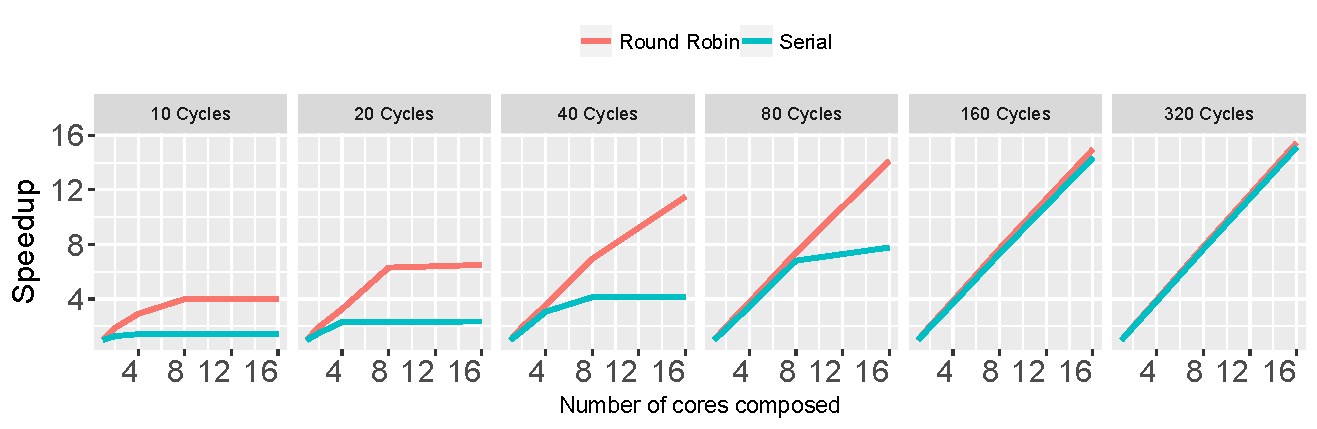
\includegraphics[width=1\textwidth]{chapter3/graphics/motivation_fetch.pdf}
    \caption{Speedup obtained when executing the synthetic block with varying execution times (facets) with the current fetching technique and new fetching technique. Higher is better.}
    \label{fig:new_fetch_ex}
\vspace{1em}
	\end{figure}

Figure~\ref{fig:motivation_fetch} illustrates how a new fetching mechanism can improve the performance of core composition, especially on small blocks that can execute quickly.
The figure shows the speedup obtained via core composition when executing a synthetic block.
The synthetic block is only four instructions long using a custom instruction whose execution time is defined ahead of the simulation; these execution times are represented by the facets, and is executed 100000 times.
The reason a four instruction block was chosen is due to the fact that it allows for four blocks to be fetched on each core.
Recalling Chapter~\ref{chp:cases}, on average block-sizes were under 32 instructions long, thus each core needs to fetch four blocks before submitting a fetch request to another core.
The colours represent the different fetching schemes, "Old" being the fetching scheme described in more detail in Chapter~\ref{chp:Background} and used in Chapters~\ref{chp:streamit} and ~\ref{chp:cases}, whilst new defines the fetching mechanism which will be described in more detail later on.

The results in the figure show that unless a block is at least 80 cycles long, it is difficult to efficiently use 16 core compositions using the normal fetching scheme.
To give a point of reference -- using data gathered from the SD-VBS benchmarks from Chapter~\ref{chp:cases} -- the average execution time of a block in SD-VBS is 20 cycles long.
However, with the new fetching scheme, 16 cores becomes useful when blocks are at least 40 cycles long, enabling a 3x speedup compared to the old fetching scheme.
For smaller core compositions, such as 2 and 4 fused cores, using a different fetching scheme from the traditional method allows for core composition to speedup execution when blocks are even 10 cycles long.
